\documentclass[a4paper]{article}

% Packages.
\usepackage{amsmath}
\usepackage{amsthm}
\usepackage[answerdelayed]{exercise}
\usepackage[usenames,dvipsnames]{color}

% Definitions.
\theoremstyle{definition}
\newtheorem{definition}{Definition}

\renewcommand{\ExerciseHeader}{\vspace{7mm}\par\noindent\textbf{\large
\ExerciseName\ \ExerciseHeaderNB\ExerciseHeaderTitle
\ExerciseHeaderOrigin}\par}

\renewcommand{\AnswerHeader}{\par\noindent\textbf{
Answer of \ExerciseName\ \ExerciseHeaderNB}\par}

% Options.


\title{The analysis of variance}
\author{Guillaume Filion}
\usepackage{Sweave}
\begin{document}
\maketitle


%% The problem %%
\section{The problem}

In 1992, Denke and Grundy set out to study the effect of different
insaturated fats in the diet on the total blood cholesterol. They
controlled the diet of 15 patients with the same amount of insaturated
fats of different kinds. Here is what they obtained (the study is real
but the data is fake).

\begin{center}
  Total blood cholesterol (mmol/L)
  \par
  \begin{tabular}{ccc}
      High oleic & High lauric & High palmitic \\\hline
      3.08 & 3.75 & 2.83 \\ 
      5.71 & 5.13 & 3.91 \\
      5.28 & 5.74 & 6.46 \\
      5.26 & 3.22 & 7.34 \\
      4.44 & 5.51 & 6.36 \\
  \end{tabular}
\end{center}

In your \texttt{R} session, manually enter the data in 3 vectors of
length 5 (\texttt{oleic}, \texttt{lauric}, \texttt{palmitic}).

\begin{Schunk}
\begin{Sinput}
> oleic <- c(3.08, 5.71, 5.28, 5.26, 4.44);
> lauric <- c(3.75, 5.13, 5.74, 3.22, 5.51);
> palmitic <- c(2.83, 3.91, 6.46, 7.34, 6.36);
\end{Sinput}
\end{Schunk}

\begin{Exercise}
Can we assume that the data is Gaussian? What is the null hypothesis
in that case?
\end{Exercise}
\begin{Answer}
Yes, we can assume that the data is Gaussian. Medical `reaction norms'
often have a Gaussian distribution.
The null hypothesis resembles that of the $t$ test. The only difference
is that we have more than one population.
\begin{enumerate}
\item
All datasets are sampled from a Gaussian distribution.
\item
\label{reject}
The parameters are unknown, but equal in all cases.
\item
Sampling is IID.
\end{enumerate}
\end{Answer}

\begin{Exercise}
What are the risks of doing 3 $t$ tests? Find a statistic $F$ that allows
you to do a single test. Formulate the null hypothesis.
\end{Exercise}
\begin{Answer}
The risks of doing several $t$ tests are that the power will be low
(because we will not use all the samples in each test) and that we
will need to correct for multiple testing (and the tests
are not independent by the way).

A good test statistic is the ratio of the variance of the means to the
mean of the variances. For simplicity, we drop the normalization constants
and work with the sum of squares instead.

\begin{equation}
F = \frac{\sum_{i=1}^3 \sum_{j=1}^5 (\bar{x}_i - \bar{x})^2}
  {\sum_{i=1}^3 \sum_{j=1}^5 (x_{ij} - \bar{x}_i)^2}
\end{equation}

It is associated with the alternative hypothesis
in which the item \ref{reject} is replaced by `At least two samples
are taken from distributions with a different mean'.
\end{Answer}


%% The test statistic %%
\section{The test statistic}

As usual, we need to make our life easier by writing a function to
compute the statistic. Then we resample the statistic under the
null hypothesis.

\begin{Exercise}
Write a function that computes the $F$ statistic. Assume that the
input is a \texttt{list} of vectors. Try to write a function that would
work for any number of samples, not just 3.
\end{Exercise}
\begin{Answer}
\begin{Schunk}
\begin{Sinput}
> F <- function(samplist) {
+   grandmean <- mean(unlist(samplist));
+   num <- 0;
+   denom <- 0;
+   for (smpl in samplist) {
+     # Terms in j are ientical in numerator of formula (1).
+     num = num + length(smpl)*(mean(smpl)-grandmean)^2;
+     # Compute sum of squares as (n-1)*var.
+     denom = denom + (length(smpl)-1)*var(smpl);
+   }
+   return (num/denom);
+ }
> F.obs <- F(list(oleic, lauric, palmitic));
> F.obs;
\end{Sinput}
\begin{Soutput}
[1] 0.06273586
\end{Soutput}
\end{Schunk}
\end{Answer}

\begin{Exercise}
Using the function to compute the $F$ statistic or from the formula,
prove that $F$, like the effect size $t$ is invariant by translation
and scaling. What does that mean for the resampling?
\end{Exercise}
\begin{Answer}
The demonstration is essentially the same as the one shown for the $t$
statistic. We can verify it with a few examples.
\begin{Schunk}
\begin{Sinput}
> F(list(oleic+1, lauric+1, palmitic+1));
\end{Sinput}
\begin{Soutput}
[1] 0.06273586
\end{Soutput}
\begin{Sinput}
> F(list(pi*oleic+1, pi*lauric+1, pi*palmitic+1));
\end{Sinput}
\begin{Soutput}
[1] 0.06273586
\end{Soutput}
\end{Schunk}
This means that we can resample $F$ with standard Gaussian variables,
because all Gaussian variables will have the same distribution of $F$
under the null hypothesis.
\end{Answer}

\begin{Exercise}
Resample $F$ under the null hypothesis. Find estimates of the limits of
the rejection region. Finish the test. Estimate the p-value.
\end{Exercise}
\begin{Answer}
\begin{Schunk}
\begin{Sinput}
> F.smpl <- rep(NA, 10000);
> for (i in 1:10000) {
+   F.smpl[i] <- F(list(rnorm(5), rnorm(5), rnorm(5)));
+ }
> plot(density(F.smpl), main="Density of F", xlab="Value");
> # Note that the rejection region is necessarily unilateral.
> abline(v=F.obs, col=2);
> quantile(F.smpl, probs=0.95);
\end{Sinput}
\begin{Soutput}
      95% 
0.6503363 
\end{Soutput}
\begin{Sinput}
> # Not significant. Let's have a look at the p-value.
> mean(F.smpl >= F.obs);
\end{Sinput}
\begin{Soutput}
[1] 0.6896
\end{Soutput}
\end{Schunk}
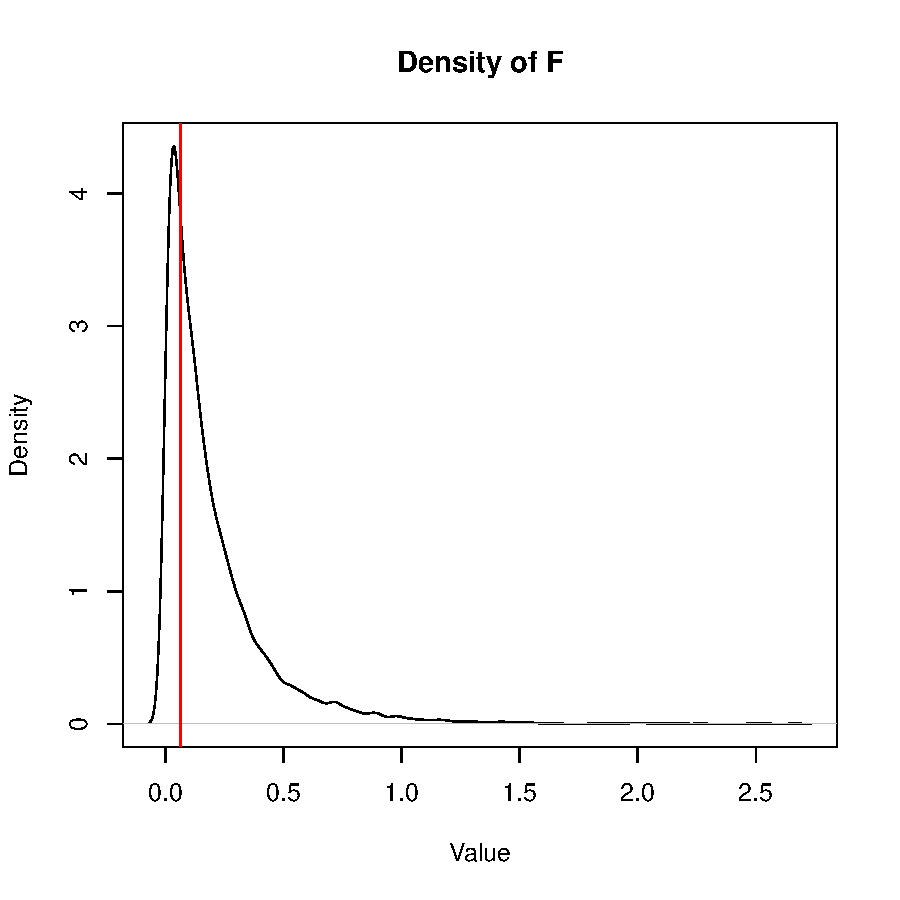
\includegraphics{anova-004}
\par
Note that the distribution of $F$ is not symmetric. If $F$ is small,
all the samples have similar means and we do not want to reject the null
hypothesis. We reject it only when $F$ is large, so in the analysis of
variance, the test is only one-sided.
\end{Answer}

\begin{Exercise}
Compare your results with that of \texttt{R}. The way to do an ANOVA
in \texttt{R} is not very intuitive. You need to put all the observations
in a single vector, say \texttt{obs}, build a \texttt{factor} that
indicates which sample they belong to, say \texttt{smpl} and use
\texttt{anova(lm(obs \~\ smpl))}.
\end{Exercise}
\begin{Answer}
\begin{Schunk}
\begin{Sinput}
> obs <- c(oleic, lauric, palmitic);
> smpl <- factor(rep(c("oleic", "lauric", "palmitic"), each=5));
> anova(lm(obs ~ smpl));
\end{Sinput}
\begin{Soutput}
Analysis of Variance Table

Response: obs
          Df  Sum Sq Mean Sq F value Pr(>F)
smpl       2  1.5051 0.75253  0.3764 0.6941
Residuals 12 23.9903 1.99919               
\end{Soutput}
\end{Schunk}
\par
Again, the $F$ used by \texttt{R} is not the same as the one we have used
(it varies only by a scaling factor), but the p-value, indicated in the
column \texttt{Pr(>F)} is close to the one we found.
\end{Answer}


\cleardoublepage
\shipoutAnswer
\end{document}

